\documentclass[11pt,a4paper]{article}
\usepackage[T1]{fontenc}
\usepackage{lmodern}
\usepackage[utf8]{inputenc}
\usepackage[margin=1in]{geometry}
\usepackage{amsmath,amssymb,bm,booktabs,microtype}
\usepackage{tikz}
\usetikzlibrary{arrows.meta}
\usepackage[colorlinks=true,linkcolor=blue,urlcolor=blue]{hyperref}
\title{Interpreting Inverse Dynamics in Two-Handed Golf Swing Analysis:\\Wrenches, Contact Allocation and Mechanical Power}
\author{Dieter Olson}
\date{Revised September 8, 2026}
\begin{document}\maketitle
\begin{abstract}
A recovered hand wrench constrains the combined mechanical action of the hands. It does not generally determine their individual force distributions or muscle recruitment. This technical companion derives the origin transformation, a physically valid contact null-space example, and the invariance of total wrench power. It also states when actuator inputs are unique and why subtracting drift twice is an error. The aim is to retain the useful information in inverse dynamics while preventing a torque component from becoming an unsupported instruction to twist the club.
\end{abstract}

\section{Recover the Hand Wrench in One Frame}
Take the club as a rigid body in a fixed right-handed inertial frame. Let $C$ be its center of mass, $I_C$ its consistently expressed inertia tensor, and $P$ a reporting point on the grip. If $F_a,M_{a,C}$ denote known non-hand, non-gravitational external loads, then
\begin{align}
F_h&=ma_C-mg-F_a,\\
M_{h,C}&=I_C\alpha+\omega\times(I_C\omega)-M_{a,C},\\
M_{h,P}&=M_{h,C}+(r_C-r_P)\times F_h.\label{eq:recover}
\end{align}
Uniform gravity has no moment about $C$. Include ball and turf loads when present; without their values, motion does not uniquely separate them from hand loads. The equations describe hand-on-club action; reversing to club-on-hand action reverses the wrench at the same point.

The rotational expression is a rigid-body approximation. Shaft deformation may require segment or distributed momentum balances. A high sampling rate does not itself validate the required accelerations: filtering, motion noise, calibration, synchronization and uncertain inertias affect the result. A smooth preimpact reconstruction does not resolve collision forces merely because it can be evaluated at the nominal impact time.

\section{Derive the Reference Transformation}
For forces $F_i$ at $r_i$ and local couples $C_i$, the moment about $P$ is
$M_P=\sum_i[(r_i-r_P)\times F_i+C_i]$. Therefore
\begin{align}
M_Q-M_P
&=\sum_i(r_P-r_Q)\times F_i\\
&=(r_P-r_Q)\times F,
\end{align}
where $F=\sum_iF_i$. This establishes both the sign and the fact that the \emph{same} force must be used in the transform. Rotating the axes additionally requires rotating both vectors into the new basis. Translating the wrench is distinct from writing angular momentum about a moving point; the latter requires the appropriate transport terms.

A pure couple has zero resultant and does not change with reference. The moment component of a wrench with nonzero resultant generally does. Moving the force to $Q$ requires a changed accompanying couple; a free couple in the original representation is not an excuse to keep both components unchanged.

Take $P=0$, $A=(0.5,0,0)$ m and $F=(0,4,0)$ N. The wrench about $P$ is $F$ and $M_P=(0,0,2)$ N m. A force at $P$ plus that couple is equivalent to the original force at $A$. A pure couple alone is not: it lacks the $4$ N resultant. An offset force has a real rotational effect even when there is no independently applied local contact couple.

\begin{figure}[htbp]\centering
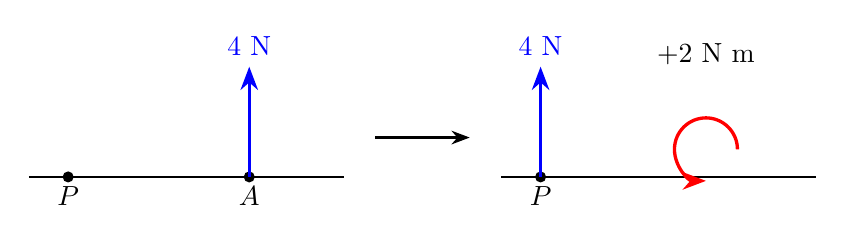
\begin{tikzpicture}[>=Stealth]
\draw[thick] (0,0)--(4,0);\fill(.5,0) circle(2pt);\fill(2.8,0) circle(2pt);
\node[below] at(.5,0){$P$};\node[below] at(2.8,0){$A$};
\draw[->,very thick,blue] (2.8,0)--(2.8,1.4) node[above]{$4$ N};
\draw[->,thick] (4.4,.5)--(5.6,.5);
\draw[thick] (6,0)--(10,0);\fill(6.5,0) circle(2pt);\node[below] at(6.5,0){$P$};
\draw[->,very thick,blue] (6.5,0)--(6.5,1.4) node[above]{$4$ N};
\draw[->,very thick,red] (9,.35) arc(0:270:.4);
\node[above] at(8.6,1.3){$+2$ N m};
\end{tikzpicture}
\caption{Alternative Representations With Identical Resultant and Moment. Positive Moment Is Counterclockwise.}
\end{figure}

\section{A Coordinate Range Is Not a Load-Sharing Estimate}
For $F=(0,F_y,0)$ and $Q=(s,0,0)$ relative to $P$, the exact planar rule is
$M_{Q,z}=M_{P,z}-sF_y$. Chosen values $F_y=40$ N and $M_{P,z}=2$ N m give
\begin{center}\begin{tabular}{rrrr}\toprule
$s$ (m) & $-0.10$ & $0$ & $+0.10$\\
$M_{Q,z}$ (N m) & $6$ & $2$ & $-2$\\\bottomrule
\end{tabular}\end{center}
The sign change does not identify a positive couple at one hand and a negative couple at the other. These are three reports of the same aggregate wrench. Their range is not a confidence interval, and a percentage change becomes unstable near a zero denominator.

For a three-dimensional wrench with $F\ne0$, $F\cdot M_P$ is invariant under translation. A zero-moment application point exists only when $F\cdot M_P=0$; even then its line of action need not intersect the grip. Thus a general hand wrench cannot always be replaced by a single force at a presumed pressure center. Distributed tractions may produce a residual torsional couple.

\section{Contact Redundancy Has a Specific Null Space}
For two contacts with forces $F_1,F_2$ and couples $C_1,C_2$,
\begin{equation}
F_h=F_1+F_2,\qquad
M_{h,P}=\sum_{i=1}^2[(r_i-r_P)\times F_i+C_i].
\end{equation}
These define a grasp map $w_h=\mathcal G\lambda$ at a fixed configuration. Internal load additions invisible to the rigid club wrench lie in $\ker\mathcal G$. This is not an unspecified ``null space of the Jacobian'': a kinematic Jacobian, its transpose and a grasp map have different domains and physical meanings.

With zero local couples and distinct contact points, let $e$ be the unit vector from contact 1 to contact 2. The additions $\delta F_1=ke$ and $\delta F_2=-ke$ have zero resultant and zero moment. Opposite forces perpendicular to that line generally form a nonzero couple; equal-and-opposite forces are not automatically invisible.

The two-point force-only grasp map has rank five. A residual moment component along the contact line cannot be freely supplied by those two point forces. Allowing local couples changes that constraint. Friction, compression, finite contact area and torque limits further restrict physically admissible solutions. There is no universal count of unidentified loads that applies to every grip model.

For a consistent wrench, $\lambda=\mathcal G^+w_h+n$ with $n\in\ker\mathcal G$ describes an algebraic family. A chosen metric and regularizer select an allocation, not an observation of the nervous system. Force/moment scaling must be declared when minimizing such a norm. Instrumented grip and distributed contact measurements can reduce the family; club motion alone cannot usually do so.

The arms, torso and club complete the bimanual closed chain. Loop constraints can create redundant load paths, but affine dependence on input alone does not prove nonuniqueness. A fully actuated model can have a unique net input for an observed full trajectory while still admitting many muscle or hand allocations.

\section{Inverse Dynamics Already Includes Its Bias Model}
In independent coordinates, use
\begin{equation}
M\ddot q+h=Bu+Q_{\rm ext},\qquad
\tau_{\rm ID}=M\ddot q+h-Q_{\rm ext}=Bu.
\end{equation}
Defining $a_d=M^{-1}(Q_{\rm ext}-h)$ gives
$\tau_{\rm ID}=M(\ddot q-a_d)$. No second drift subtraction is needed. The first-order affine form for $x=(q,\dot q)$ has drift $(\dot q,a_d)$ and input gain $(0,M^{-1}B)$.

For a pendulum with $m=1$ kg, $L=1$ m, $g=9.81$ m/s$^2$ and $q=30^\circ$ from downward vertical, zero pivot torque gives $\ddot q=-4.905$ rad/s$^2$. Inverse dynamics returns zero, because its acceleration and gravity terms cancel. A stationary hold at that angle instead requires $4.905$ N m. This separates the applied torque from the acceleration resultant with a directly checkable example.

If $B$ has full column rank and the recovered load lies in its image, the modeled input is unique. Redundancy introduces $\ker B$; a nonzero consistency residual can indicate measurement error, omitted loads or model inadequacy. A net joint torque containing unmodeled passive tissue forces is not a uniquely identified muscle command.

In constrained coordinates, reaction forces generally depend on actuation. A zero-actuator motion can have nonzero reactions, but their entire history cannot simply be designated input-independent drift. Eliminating the constraints changes both drift and input gain. Similarly, a zero-net-torque simulation is not automatically an experiment in physiological relaxation.

\section{Power Provides an Invariant Check}
For material points of a rigid club,
$v_Q=v_P+\omega\times(r_Q-r_P)$. Combining this with the wrench transform gives
\begin{equation}
F_h\cdot v_P+M_{h,P}\cdot\omega
=F_h\cdot v_Q+M_{h,Q}\cdot\omega.
\end{equation}
For the $4$ N example, let $v_P=0$ and $\omega=(0,0,2)$ rad/s. At $A$, $v_A=(0,1,0)$ m/s and force power is $4$ W. At $P$, the same power appears entirely as moment power: $2$ N m times $2$ rad/s. The force and couple percentages change, but total hand power does not.

At a flexible interface, use the actual local velocities and include deformation power. Total mechanical power also does not measure metabolic effort. Co-contraction and isometric contact force can be substantial while net external power is small. In a fixed-pivot circular example, an inward contact load supplies centripetal acceleration with zero instantaneous force power; it is a real transmitted force, not a fictitious load to subtract before estimating sensation.

\section{Omitted Loads and a Defensible Interpretation}
If aerodynamic loading is omitted while motion is fixed, the no-aerodynamics inference differs from the corrected hand wrench by $(F_a,M_{a,P})$ at the same reporting point. Its correction can increase or decrease a signed component. Drag direction is defined relative to airflow, while lift, aerodynamic moment and coordinate projection require separate treatment. A driver study does not establish a universal iron correction.

For an analysis labelled ``alpha torque,'' state the origin, basis, positive axis, action convention and whether the output is a wrench projection or generalized torque. A torque sign alone does not reveal total power, hand allocation, muscle effort or the merit of a coaching cue. Earlier work, evolving geometry, shaft energy and changing contact conditions are intertwined through the state.

Use the recovered wrench to constrain a mechanistic hypothesis. Then test contact feasibility, propagate uncertainty and compare independent measurements. A forward/inverse round trip checks consistency of one model; independent load measurements test an additional claim. A useful result reports both what was identified and which extra measurement would distinguish the remaining explanations.

\section*{References and Companion}
The wrench, dynamics and contact conventions follow K. M. Lynch and F. C. Park, \emph{Modern Robotics} (Cambridge University Press, 2017), Chapters 3, 8 and 12, and R. Featherstone, \emph{Rigid Body Dynamics Algorithms} (Springer, 2008). The longer companion, \emph{Interpretation of Inverse Dynamics: Understanding the Fundamental Limitations}, contains the constrained-reaction derivation, signed aerodynamic worked cases and a complete evidence plan. Wrench supplement: \url{https://modernrobotics.northwestern.edu/nu-gm-book-resource/3-4-wrenches/}.
\end{document}
